\subsection{Home Module}
\label{sec:mobile-home}

\textbf{Purpose:}
Serves as the primary landing page of the Floo mobile application after successful authentication. The Home module provides users with quick access to project management features, workflow shortcuts, and a summary of recent activities through a responsive and user-friendly interface.

\vspace{0.2cm}
\noindent\textbf{Main Features}

\begin{itemize}
    \item Personalized Welcome Section
    \item Quick Project Actions
    \item Workflow Overview
    \item Recent Activities
    \item Bottom Navigation
\end{itemize}

%%%%%%%%%%%%%%%%%%%%%%%%%%%%%%%%%%%%%%%%%%%%%%%%%%%%%%%%%%%%

\subsubsection{Dynamic Home Hub}

\textbf{Purpose:}
Provides a personalized dashboard that enables users to access the application's core features immediately after logging in.

\begin{figure}[H]
    \centering
    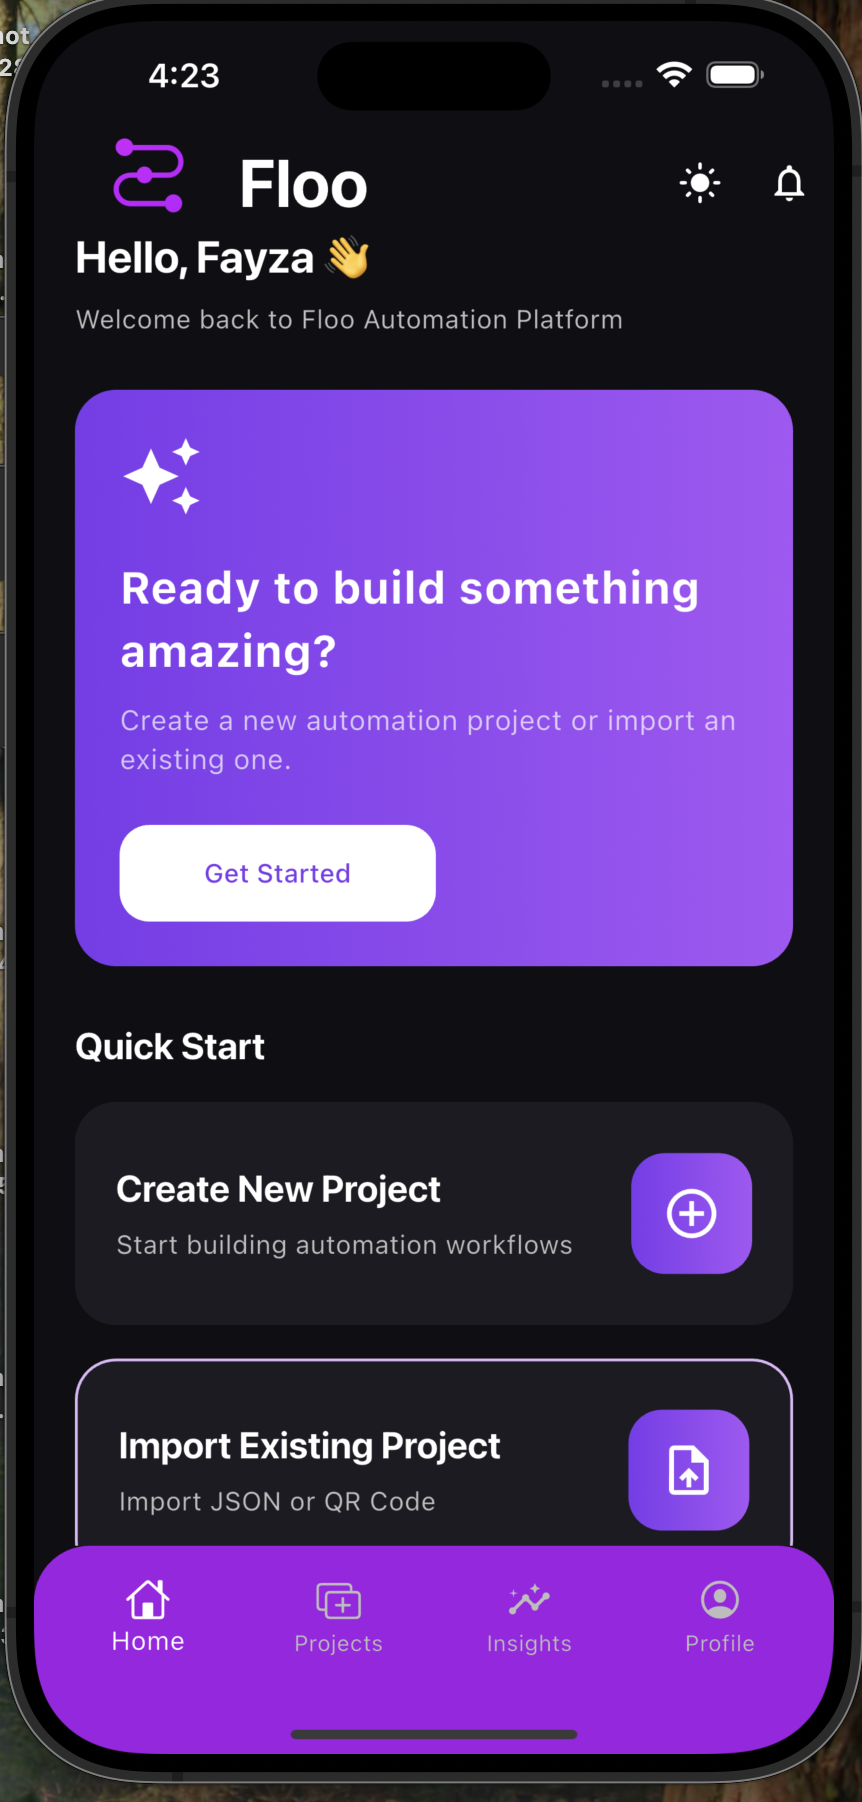
\includegraphics[width=0.42\textwidth]{images/mobile-app/admin-dashboard/home-page-1-D.png}
    \caption{Dynamic Home Hub}
    \label{fig:mobile-home}
\end{figure}

\vspace{0.2cm}
\noindent\textbf{Main Components}

\begin{itemize}
    \item Personalized Greeting
    \item Quick Start Section
    \item Create New Project
    \item Import Existing Project
    \item Bottom Navigation Bar
\end{itemize}

\vspace{0.2cm}
\noindent\textbf{Behavior \& Logical Flows}

\begin{itemize}
    \item Displays a personalized greeting using the authenticated user's profile information.
    \item Provides quick shortcuts for creating new workflow projects.
    \item Allows users to import existing workflow configurations using JSON files or QR codes.
    \item Enables navigation between the application's main modules through the bottom navigation bar.
    \item Retrieves dashboard information immediately after successful authentication.
\end{itemize}

%%%%%%%%%%%%%%%%%%%%%%%%%%%%%%%%%%%%%%%%%%%%%%%%%%%%%%%%%%%%

\subsubsection{Operational Overview}

\textbf{Purpose:}
Provides users with a summarized overview of workflow activities, enabling them to monitor the current state of their automation projects.

\begin{figure}[H]
    \centering
    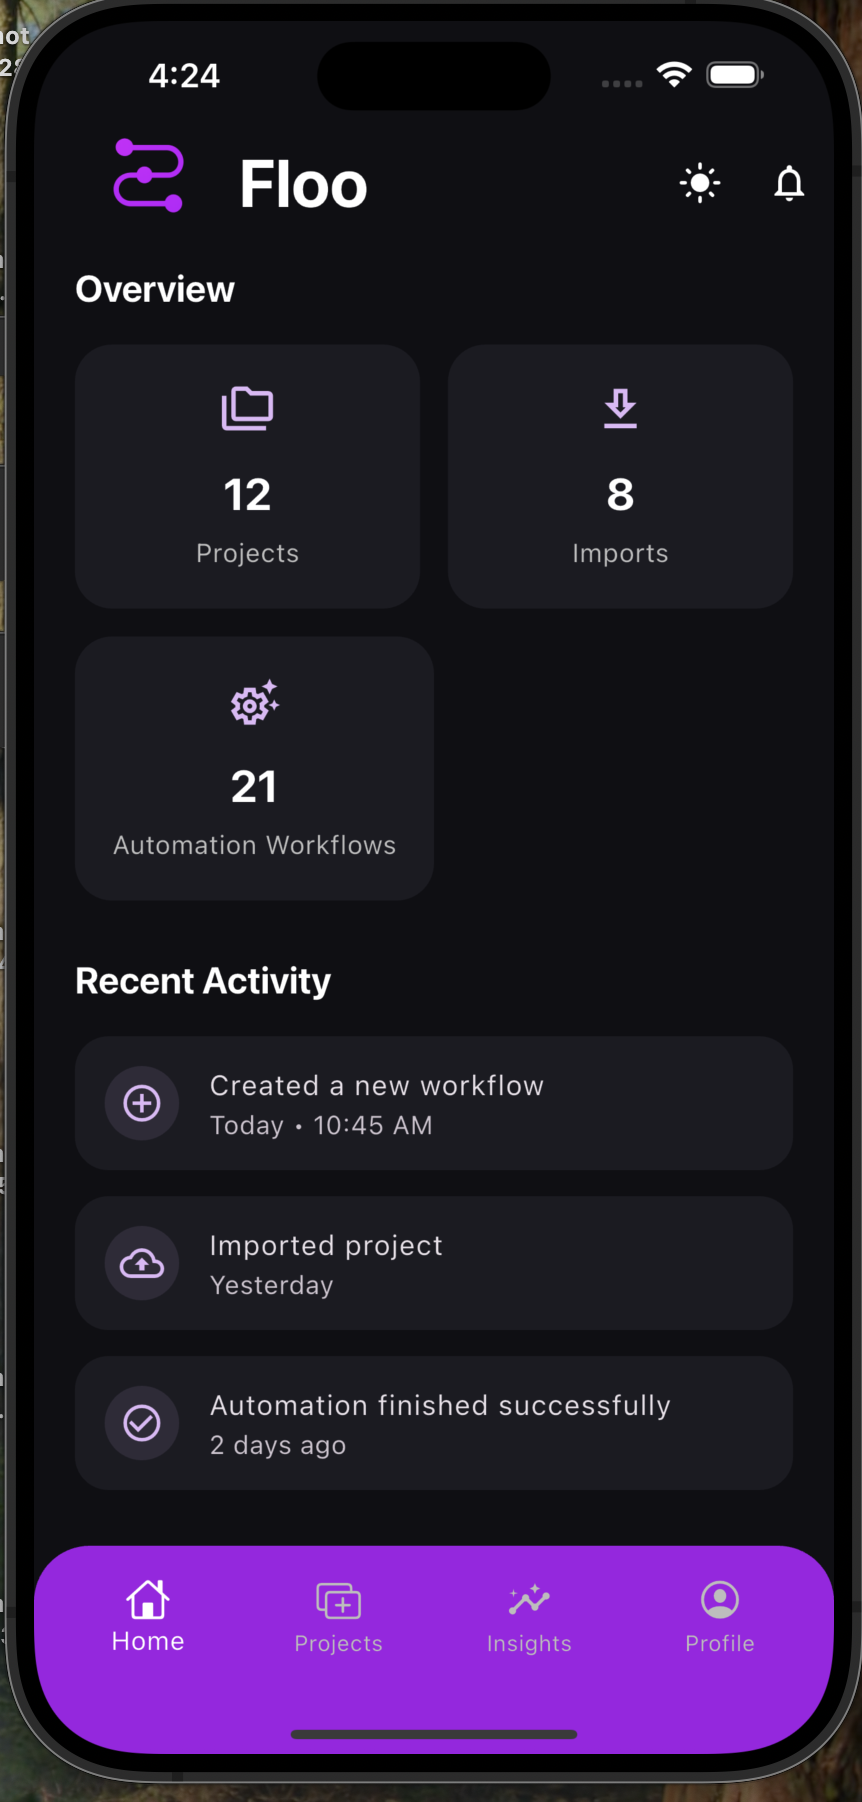
\includegraphics[width=0.42\textwidth]{images/mobile-app/admin-dashboard/home-page-2-D.png}
    \caption{Operational Overview}
    \label{fig:mobile-home-overview}
\end{figure}

\vspace{0.2cm}
\noindent\textbf{Main Components}

\begin{itemize}
    \item Workflow Statistics
    \item Recent Activities
    \item Running Workflows Summary
    \item Project Overview Cards
\end{itemize}

\vspace{0.2cm}
\noindent\textbf{Behavior \& Logical Flows}

\begin{itemize}
    \item Retrieves workflow statistics from the backend through authenticated REST API requests.
    \item Displays project summaries and workflow information in an organized layout.
    \item Presents recent workflow activities to keep users informed of the latest operations.
    \item Refreshes dashboard information whenever the page is reloaded.
    \item Provides visual indicators representing the operational status of workflow projects.
\end{itemize}

%%%%%%%%%%%%%%%%%%%%%%%%%%%%%%%%%%%%%%%%%%%%%%%%%%%%%%%%%%%%

\subsubsection{Navigation Flow}

\textbf{Purpose:}
Provides seamless navigation between the primary modules of the mobile application through a persistent bottom navigation bar.

\vspace{0.2cm}
\noindent\textbf{Navigation Items}

\begin{itemize}
    \item Home
    \item Projects
    \item Analytics
    \item Profile
\end{itemize}

\vspace{0.2cm}
\noindent\textbf{Behavior \& Logical Flows}

\begin{itemize}
    \item Preserves the selected screen while navigating between application modules.
    \item Highlights the currently active navigation item.
    \item Enables quick access to the application's core features.
    \item Maintains a consistent navigation experience throughout the application.
\end{itemize}

%%%%%%%%%%%%%%%%%%%%%%%%%%%%%%%%%%%%%%%%%%%%%%%%%%%%%%%%%%%%

\subsubsection{Home Data Loading}

\textbf{Purpose:}
Ensures that the Home screen always displays the latest workflow information synchronized with the backend.

\vspace{0.2cm}
\noindent\textbf{Behavior \& Logical Flows}

\begin{itemize}
    \item Sends authenticated API requests using the stored JWT access token.
    \item Retrieves user profile information after authentication.
    \item Fetches workflow statistics and recent activities from the backend.
    \item Displays loading indicators while waiting for server responses.
    \item Handles communication errors gracefully by displaying appropriate feedback messages.
\end{itemize}